Neste capítulo, apresentamos os fundamentos da Análise de Redes Sociais. A análise de redes sociais (ARS) é uma abordagem que tem suas raízes na Sociometria e na Teoria dos Grafos, que são de viés matemático, para analisar relações sociais \cite{2015_Recuero_BOOK}. A ideia central é que os indivíduos, ou atores sociais, estão inseridos em estruturas complexas de relações com outros atores, e essas estruturas têm um papel fundamental no comportamento e na visão de mundo desses indivíduos. 

A partir da base teórica, apresentamos as câmaras de eco comparando alguns estudos de caso e apresentando a metodologia de \citeonline{2023_Atiqi_BOOK} para simulação de câmaras de eco em redes de compartilhamento de notícias. Essa metodologia, baseada na Modelagem Baseada em Agentes é analisada no fim do capítulo, após uma após apresentarmos a Analise de Sentimento como um insumo adicional na análise de redes.

\section{Teoria dos Grafos}
A Teoria dos Grafos é um framework matemático que estuda as relações entre objetos e as conexões entre eles \cite{1986_Biggs_BOOK}. As origens desta teoria estão no trabalho do matemático Euler e na solução que ele propôs para o enigma das Pontes de Königsberg, conforme traduzido por \citeonline{2020_Lopes}. A história relata que a cidade de Königsberg seria atravessada por sete pontes e que popularmente havia um desafio de desenhar um caminho por ela onde cada uma das pontes seria atravessada uma única vez. Euler teria demonstrado que tal desafio era impossível de ser resolvido utilizando um grafo, dando assim origem à teoria.

Em \citeonline{2017_Recuero}, a autora discute a importância da ARS e da Teoria dos Grafos para a compreensão das redes sociais online. Ela explica que a ARS permite a análise sistemática de grupos sociais a partir de sua estrutura, através de medidas específicas. A autora também destaca que a análise de redes sociais nasce de um ramo interdisciplinar de pesquisa, cujas bases podem ser encontradas nas mais variadas ciências, principalmente no início do século XX, particularmente, a partir da década de 1930.

Um conceito fundamental na Teoria dos Grafos é o de um "grafo", que é uma estrutura composta por "vértices" (ou "nós") e "arestas" que conectam esses vértices. Formalmente, segundo \citeonline{1976_Bondy_BOOK} um grafo $G$ é definido como um par ordenado $G := (V, E)$ compreendendo um conjunto $V$ de vértices ou nós juntamente com um conjunto $E$ de arestas ou arcos, que são pares de vértices.

Os grafos podem ser categorizados como direcionados ou não direcionados. Em um grafo direcionado, as arestas têm uma direção associada, indicando uma relação unidirecional. Em contraste, em um grafo não direcionado, as arestas não têm direção, sugerindo uma relação bidirecional \cite{2000_West_BOOK}. Em termos de redes sociais, um exemplo de grafo direcionado seria o Twitter (onde um usuário pode seguir outro sem ser seguido de volta), enquanto um exemplo de grafo não direcionado seria o Facebook (onde a amizade é sempre mútua).

\begin{figure}
	\centering
	\begin{tikzpicture}[node distance=2cm]

		% Estilos para os nós e arestas
		\tikzstyle{user} = [circle, draw=black, fill=blue!30, minimum size=1cm, inner sep=0pt]
		\tikzstyle{follow} = [thick,->,>=stealth]

		% Usuários
		\node (A) [user, label=below:Ana] {};
		\node (B) [user, right=of A, label=below:Bob] {};
		\node (C) [user, above right=of A, label=right:Carlos] {};
		\node (D) [user, below right=of A, label=right:Diana] {};
		\node (E) [user, below=of D, label=below:Eva] {};
		\node (F) [user, left=of E, label=below:Felipe] {};
		\node (G) [user, above left=of F, label=left:Gabriel] {};

		% Relações de "seguir"
		\draw[follow] (A) -- (B);
		\draw[follow] (B) -- (C);
		\draw[follow] (C) -- (D);
		\draw[follow] (D) -- (A);
		\draw[follow] (A) -- (C);
		\draw[follow] (B) -- (D);
		\draw[follow] (E) -- (D);
		\draw[follow] (E) -- (F);
		\draw[follow] (F) -- (G);
		\draw[follow] (G) -- (A);

	\end{tikzpicture}
	\caption{Ilustração de uma rede social com usuários seguindo uns aos outros. O subgrafo formado por Ana, Bob, Carlos e Diana representa um clique, pois todos estão conectados entre si. O caminho de Eva para Ana passa por Diana e Gabriel.}
\end{figure}

Outro conceito importante é o "grau" de um vértice, que é o número de arestas conectadas a ele. Em um grafo direcionado, distinguimos entre o "grau de entrada" (o número de arestas que entram no vértice) e o "grau de saída" (o número de arestas que saem do vértice). O grau de um vértice pode ser usado para medir sua importância ou influência dentro da rede \cite{2010_Newman_BOOK}.

Um "caminho" em um grafo é uma sequência de vértices na qual cada vértice é conectado ao próximo por uma aresta. O "comprimento" de um caminho é o número de arestas que ele contém. Este conceito é crucial para entender como a informação ou influência pode se propagar através da rede \cite{2010_Easley_BOOK}.

A "conectividade" de um grafo é uma medida de quão integrada ou unida é a rede. Um grafo é dito "conectado" se houver um caminho entre cada par de vértices \cite{2000_West_BOOK}.

Um "subgrafo" é um grafo formado a partir de um conjunto de vértices e arestas de um grafo maior. Os subgrafos podem ser usados para estudar partes específicas de uma rede \cite{2000_West_BOOK}.

\citeonline{2017_Recuero} também enfatiza a diferença entre redes sociais e sites de rede social. Enquanto uma rede social está relacionada à percepção de um grupo social determinado pela sua estrutura (a “rede”), que é geralmente oculta, pois só está manifesta nas interações, as ferramentas sociais na internet são capazes de publicizar e influenciar essas estruturas sociais. Assim, o Facebook, por si só, não apresenta redes sociais. É o modo de apropriação que as pessoas fazem dele que é capaz de desvelar redes que existem ou que estão baseadas em estruturas sociais construídas por essas pessoas.

Portanto, a Teoria dos Grafos e a Análise de Redes Sociais são ferramentas essenciais para a compreensão das complexas redes de interações sociais que se formam tanto no mundo offline quanto online. Elas permitem uma visão mais profunda e sistemática das relações sociais, contribuindo para uma melhor compreensão dos fenômenos sociais.

\subsection*{Grafos Sociais}

Um dos primeiros desenvolvimentos na análise de redes foi o trabalho do sociólogo Georg Simmel no início do século XX. Simmel aplicou os princípios da teoria dos grafos às relações sociais, argumentando que as estruturas sociais surgem a partir dos padrões de interação entre os indivíduos \cite[]{2021_Hollstein}. Desde então, a análise de redes tem sido aplicada em uma ampla gama de campos, incluindo ciência da computação, física, biologia e ciências sociais, entre outros.

Simmel foi pioneiro em determinar a interação social como o bloco de construção básico da sociologia. Ele argumentou que para entender o comportamento social, devemos estudar os padrões de interação, oferecendo insights penetrantes sobre a dinâmica das relações sociais. Embora Simmel nunca tenha usado o termo "rede social", muitos analistas de rede o consideram um precursor importante \cite{2018_Higgins_BOOK}.

Além disso, a análise de redes tem sido usada para entender a estrutura e a dinâmica de "redes escuras", como redes de criminosos ou terroristas. A análise de redes também tem sido aplicada para entender a estrutura e a dinâmica das organizações e como a estrutura da rede pode afetar a eficácia e a eficiência organizacional \cite{2017_Cunha}.

No entanto, apesar do rápido crescimento da análise de redes nas últimas duas décadas, as críticas à abordagem também aumentaram. Alguns críticos argumentam que a análise de redes pode ser excessivamente determinística, ignorando a agência individual e a complexidade das relações sociais \cite{1991_Scott}. Além disso, a análise de redes pode ser desafiadora devido à dificuldade de coletar dados completos e precisos sobre redes sociais.

A análise de redes sociais tem sido criticada por sua falta de consideração pelos aspectos qualitativos das redes sociais e por sua tendência a simplificar as complexidades das interações sociais \cite{2013_Gruzd}. Além disso, a análise de redes sociais é frequentemente criticada por sua falta de consideração pelos aspectos contextuais das redes sociais e por sua ênfase excessiva em padrões estruturais.

Essas críticas destacam a necessidade de abordagens mais holísticas e integradas para a análise de redes sociais, que levem em consideração tanto os aspectos quantitativos quanto qualitativos das redes sociais, bem como os contextos sociais e culturais em que essas redes estão inseridas.

A Teoria dos Grafos, nascida do problema das Pontes de Königsberg e formalizada por Euler, estabeleceu as bases para entendermos as complexas interconexões que permeiam não apenas estruturas físicas, mas também relações sociais. À medida que a sociedade evoluiu, as redes de interação humana se expandiram do tangível para o virtual, com as redes sociais online se tornando um novo território para aplicação desses princípios matemáticos.

O salto das pontes de Königsberg para os padrões de conexão no Twitter e Facebook não é apenas uma questão de escopo, mas também de complexidade. As redes sociais digitais de hoje permitem interações que Euler jamais poderia ter imaginado, mas a essência de sua abordagem permanece relevante. Assim como ele usou vértices e arestas para resolver o problema das pontes, hoje usamos esses mesmos elementos para mapear e entender a dinâmica das redes sociais.

Neste novo contexto, as interações entre usuários, as relações de seguimento e amizade, e até mesmo os padrões de compartilhamento de conteúdo podem ser modelados como grafos. As arestas representam as várias formas de interação — curtidas, comentários, retweets — e os vértices são os usuários, cada um com sua rede de conexões. Esta modelagem permite uma análise sofisticada do comportamento online, revelando desde estruturas de comunidade até a disseminação de informação e influência.

O estudo de grafos em redes sociais online transcende a análise de padrões de conexão. Abre-se a possibilidade de entender como as informações fluem, como as opiniões se formam e se polarizam, e como as comunidades online se organizam e interagem entre si. Portanto, ao aplicar a Teoria dos Grafos ao Colab, esta pesquisa busca desvendar não apenas a estrutura da rede, mas também o pulsar da participação cívica dentro dela, aplicando antigos conceitos matemáticos para resolver questões modernas de engajamento social e governança digital.

Para entender como essa disciplina pode ser aplicada ao Colab, é preciso primeiro entender o que é uma rede social online e como ela pode ser representada como um grafo. Em seguida, é preciso conhecer as principais métricas de análise de redes sociais e como elas podem ser usadas para entender o comportamento dos usuários. Por fim, é preciso entender como essas métricas podem ser aplicadas ao Colab para entender a dinâmica da participação cívica na plataforma. A seguir apresentamos algumas métricas derivativas importantes que podem ser calculadas a partir de uma lista de nós e arestas.

\subsection*{Modularidade}

\begin{figure}
	\centering
	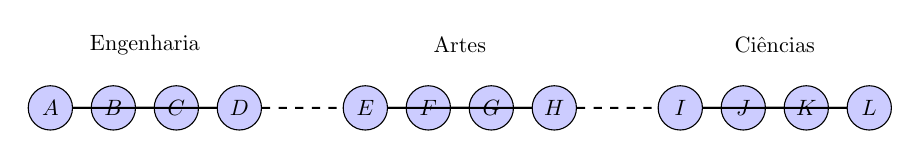
\begin{tikzpicture}[scale=0.8, every node/.style={scale=0.8}]
		% Styles
		\tikzstyle{vertex}=[circle,draw=black,fill=blue!20,minimum size=20pt,inner sep=0pt]
		\tikzstyle{edge}=[draw,thick,-]

		% Nodes for Engenharia
		\foreach \name/\x in {A/1,B/2,C/3,D/4}
		\node[vertex] (\name) at (\x,4) {$\name$};

		% Nodes for Artes
		\foreach \name/\x in {E/6,F/7,G/8,H/9}
		\node[vertex] (\name) at (\x,4) {$\name$};

		% Nodes for Ciências
		\foreach \name/\x in {I/11,J/12,K/13,L/14}
		\node[vertex] (\name) at (\x,4) {$\name$};

		% Connect nodes in Engenharia
		\foreach \source/\dest in {A/B, B/C, C/D, D/A, A/C, B/D}
		\path[edge] (\source) -- (\dest);

		% Connect nodes in Artes
		\foreach \source/\dest in {E/F, F/G, G/H, H/E, E/G, F/H}
		\path[edge] (\source) -- (\dest);

		% Connect nodes in Ciências
		\foreach \source/\dest in {I/J, J/K, K/L, L/I, I/K, J/L}
		\path[edge] (\source) -- (\dest);

		% Connect nodes between departments
		\path[edge, dashed] (D) -- (E);
		\path[edge, dashed] (H) -- (I);

		% Labels
		\node[align=center] at (2.5,5) {Engenharia};
		\node[align=center] at (7.5,5) {Artes};
		\node[align=center] at (12.5,5) {Ciências};
	\end{tikzpicture}
	\caption{Ilustração da modularidade em uma rede de estudantes de diferentes departamentos. Os nós representam estudantes, as arestas sólidas representam interações dentro dos departamentos e as arestas tracejadas representam interações entre departamentos.}
\end{figure}

A modularidade é uma métrica que quantifica a estrutura de comunidades em redes. \citeonline{2004_Newman} define a modularidade como a diferença entre a fração de arestas que caem dentro de comunidades e a fração esperada se as arestas fossem distribuídas ao acaso, mantendo a distribuição de grau dos nós. Valores de modularidade próximos a 0 indicam que a divisão da rede em comunidades não é melhor do que uma atribuição aleatória, enquanto valores próximos a 1 indicam uma divisão forte em comunidades. Em termos práticos, uma rede com alta modularidade tem mais conexões dentro de suas comunidades e menos conexões entre comunidades diferentes do que seria esperado por acaso.

Para ilustrar, imagine uma rede social de estudantes de uma universidade, onde os estudantes pertencem a diferentes departamentos, como Engenharia, Artes e Ciências. Se os estudantes de Engenharia tendem a interagir mais frequentemente entre si, e o mesmo acontece com os estudantes de Artes e Ciências, então essa rede teria uma alta modularidade. Isso porque há uma densidade maior de conexões dentro de cada departamento (comunidade) do que entre departamentos diferentes. Em contraste, se os estudantes interagissem aleatoriamente, independentemente de seus departamentos, a modularidade seria próxima de 0, indicando uma ausência de estrutura comunitária clara.

\subsection*{Centralidade e Comunidades}

Um método comum usado na análise de redes é a análise de centralidade, que mede a importância dos nós na rede com base em sua posição e conexões dentro da rede \cite[]{1978_Freeman}. Medidas de centralidade podem ajudar a identificar atores-chave na rede, ou nós que desempenham papéis importantes como porteiros, conectores ou intermediários entre diferentes partes da rede.

Outro método importante na análise de redes é a detecção de comunidades, que identifica grupos de nós que estão mais densamente conectados entre si do que com o restante da rede \cite[]{2004_Newman}. A detecção de comunidades pode ajudar a identificar grupos de indivíduos com atributos ou comportamentos semelhantes, ou grupos que são mais suscetíveis à propagação de informações ou influências.

\subsection*{Algoritmo de Louvain}

A partir dos conceitos de centralidade, comunidade e modularidade, é possivel criar heurísticas mais especializadas para interpretar os grafos das redes, por exemplo, o algoritmo de Louvain é uma metodologia heurística para detecção de comunidades em grandes redes. Desenvolvido por \citeonline{2008_Blondel}, o algoritmo tem como principal objetivo identificar grupos de nós em redes que estão mais densamente conectados entre si do que com o restante da rede. A ideia central é maximizar a modularidade da forma mais eficiente possível.

O algoritmo opera em duas fases que são repetidas iterativamente. Na primeira fase, cada nó é atribuído à sua própria comunidade. Em seguida, para cada nó, o algoritmo avalia a ganho de modularidade ao mudar a comunidade desse nó para a comunidade de seus vizinhos. Se um aumento na modularidade é observado, o nó é colocado na comunidade que proporciona esse aumento. Este processo é repetido para todos os nós até que nenhum aumento na modularidade possa ser alcançado. Na segunda fase, as comunidades encontradas na primeira fase são agregadas para formar uma nova rede de comunidades, em que os nós da nova rede representam as comunidades e os links representam as conexões entre comunidades da rede original. Estas duas fases são repetidas até que a modularidade se estabilize.

No contexto de estudos sobre câmaras de eco, o algoritmo de Louvain é particularmente relevante. Câmaras de eco são, por definição, grupos de indivíduos que compartilham e reforçam opiniões semelhantes, minimizando a exposição a opiniões divergentes. A capacidade do algoritmo de Louvain de identificar comunidades densamente conectadas em redes torna-o uma ferramenta valiosa para detectar esses grupos. Ao identificar comunidades que interagem predominantemente entre si, os pesquisadores podem isolar e estudar essas câmaras de eco, compreendendo melhor sua formação, evolução e impacto na disseminação de informações.

\section{Aplicações da Análise de Redes}

A análise de redes tem sido aplicada em uma ampla gama de campos, além das redes sociais, com aplicações que vão desde redes de transporte até a neurociência. Nesta seção, vamos destacar algumas contribuições notáveis.

No campo do transporte, a análise de redes tem sido usada para estudar o fluxo de tráfego nas estradas e identificar áreas de gargalo que podem ser melhoradas para aumentar a eficiência do tráfego \cite[]{2012_Levinson}. Por exemplo, \citeonline{2010_Bierlaire} aplicaram a análise de redes para otimizar o sistema de transporte público, reduzindo o tempo de viagem e melhorando a eficiência do serviço. No campo acadêmico, a análise de redes tem sido aplicada para estudar as redes de coautoria na publicação acadêmica. \citeonline{2001_Newman} utilizou a análise de redes para estudar os padrões de colaboração entre autores e a emergência de comunidades de pesquisa. 

No campo organizacional, a análise de redes tem sido usada para compreender a estrutura de padrões de comunicação formais e informais em organizações. \citeonline{2004_Cross_BOOK} utilizaram a análise de redes para entender como os indivíduos influenciam os processos de tomada de decisão e a emergência de estruturas de poder dentro das organizações. Na biologia, a análise de redes tem sido usada para estudar redes de interação de proteínas, redes regulatórias de genes e redes metabólicas \citeonline{2004_Barabasi} utilizaram a análise de redes para entender como as proteínas interagem entre si em uma célula, fornecendo insights sobre como as doenças afetam essas interações.

\begin{figure}[!htb]
	\caption{Imagem ilustrativa de uma rede de interação de proteínas}
	\label{fig:network_proteins}
	\centering
	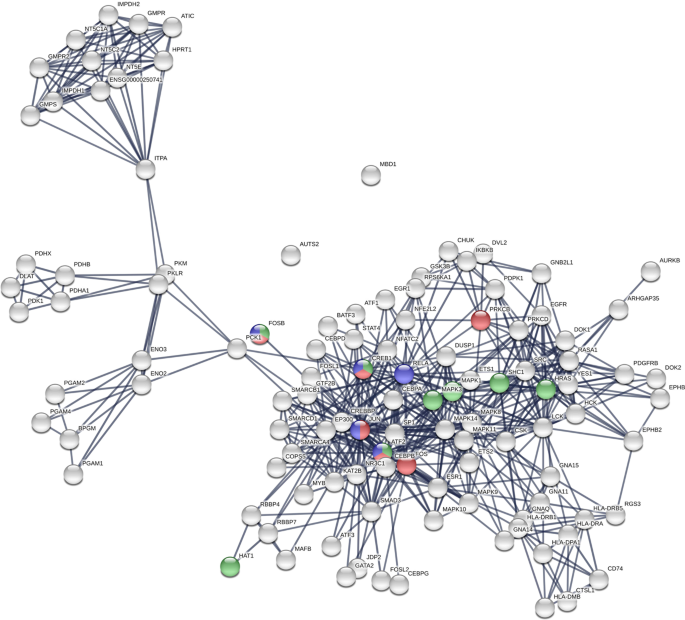
\includegraphics[scale=0.5]{images/network_proteins.png}
	\fdireta{2004_Barabasi}
\end{figure}
A análise de redes também tem sido usada em neurociência para estudar redes cerebrais. Por exemplo, pesquisadores têm utilizado a análise de redes para entender como diferentes regiões do cérebro interagem entre si, o que pode ajudar a entender doenças como a esquizofrenia e o Alzheimer \cite[]{2009_Bullmore}.
\begin{figure}[!htb]
	\caption{Imagem ilustrativa de uma rede de interação de proteínas}
	\label{fig:network_brain}
	\centering
	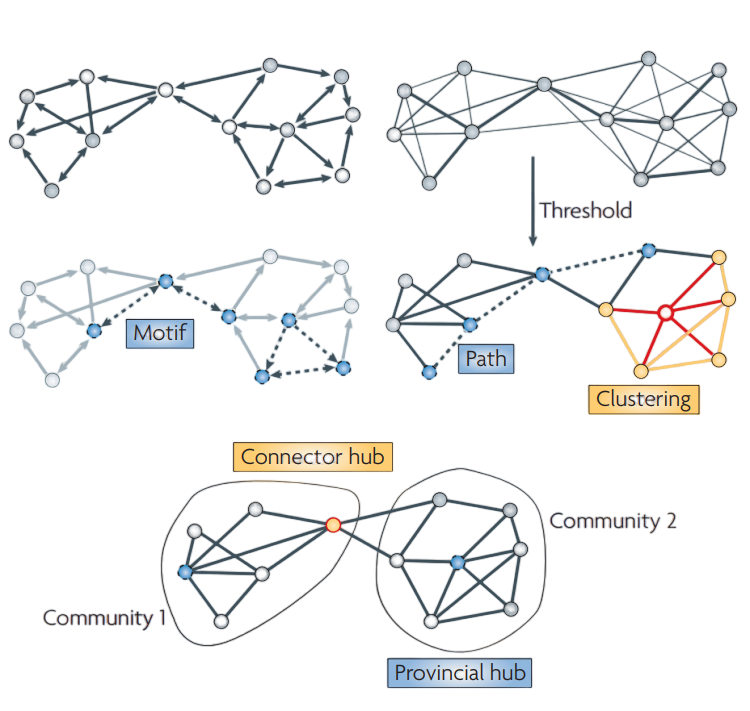
\includegraphics[scale=0.25]{images/network_brain.png}
	\fdireta{2009_Bullmore}
\end{figure}

\subsection*{Análise de Redes Sociais no Brasil}

A Análise de Redes Sociais (ARS) emergiu como uma ferramenta poderosa e cada vez mais popular para analisar a estrutura e a dinâmica das redes sociais. Utilizada para estudar uma variedade de fenômenos, como comportamento organizacional, redes políticas, crime e inovação, a ARS tem demonstrado ser uma metodologia extremamente versátil. No Brasil, a relevância da ARS é evidenciada em múltiplos contextos e áreas de estudo, incluindo o planejamento urbano, a avaliação de políticas públicas, a compreensão das dinâmicas de migração e a análise de preconceitos e divisões sociais nas redes sociais.

Um dos aspectos que torna a ARS especialmente relevante no Brasil é o alto uso de redes sociais pela população. O Brasil é um dos países com maior número de usuários de redes sociais no mundo, criando um vasto campo de dados que pode ser analisado através da ARS. Além disso, a diversidade cultural e regional do Brasil, com suas muitas diferenças locais, proporciona um cenário complexo que a ARS pode ajudar a decifrar. Ao identificar padrões de interação e circulação de informações nas redes sociais, a ARS pode revelar como essas diferenças regionais e culturais se manifestam online.

Além disso, o Brasil enfrenta uma série de questões sociais complexas e uma alta polarização política, aspectos que são frequentemente expressos e amplificados nas redes sociais. A ARS pode ser uma ferramenta valiosa para entender a formação e a dinâmica dessas polarizações, assim como para estudar a formação de grupos de opinião e a disseminação de informações (ou desinformação). Por último, eventos de grande escala, como a Copa do Mundo, as Olimpíadas ou as eleições presidenciais, geram uma enorme quantidade de atividade nas redes sociais, proporcionando oportunidades únicas para a aplicação da ARS.

Diante deste cenário, este capítulo apresenta um resumo breve da de algumas contribuições relevantes que utilizam a ARS no Brasil, começando com uma revisão de suas principais contribuições teóricas e metodológicas. Em seguida, ele discute os desafios atuais e futuros na aplicação desta abordagem no contexto brasileiro, com o objetivo de explorar como a ARS pode continuar a fornecer insights valiosos em meio à constante evolução das redes sociais.

Do ponto de vista teórico, a Análise de Redes Sociais (ARS) tem sido fundamental para entender como as redes sociais influenciam a formação de opiniões, a disseminação de informações e a mobilização social. Um exemplo relevante é o estudo de \citeonline{2021_Recuero}, que investigaram a polarização em torno do uso da cloroquina para tratar a COVID-19 no Brasil, analisando dados do Twitter. O estudo mostrou como a ARS pode ser aplicada para identificar câmaras de eco e a formação de bolhas de filtro, em que usuários com diferentes posições políticas e ideológicas têm acesso a fontes de informação divergentes. A análise revelou que a narrativa sobre a cloroquina foi capturada pela disputa política, com diferentes grupos compartilhando e reforçando suas crenças por meio das redes sociais. O trabalho de Recuero também informa a metodologia de \citeonline{2021_Kalinke} que explora a topologia da rede entre usuários do Twitter apoiadores e críticos ao governo de Jair Bolsonaro em relaçao as 100 mil mortes por COVID-19. O estudo utilizou métricas de centralidade para identificar clusters de usuários que não interagem entre membros fora das suas bolhas, o que contribui com um discurso reverberado por câmaras de eco.

Além disso, a ARS tem sido usada para investigar como as redes sociais podem facilitar a disseminação de informações falsas ou enganosas, o que tem implicações significativas para a democracia e a saúde pública. Um estudo interessante foi conduzido por \citeonline{2020_Lima}, que analisaram a circulação de informações sobre a COVID-19 no Twitter. Eles utilizaram a ARS para identificar padrões de compartilhamento de conteúdo e relacionamentos entre usuários. O estudo revelou que a desinformação estava fortemente associada ao consumo de veículos hiperpartidários e ao conteúdo de mídia social, enquanto a informação factual estava mais associada a veículos jornalísticos e institucionais. Isso demonstra como a ARS pode contribuir para a compreensão dos mecanismos de propagação da desinformação nas redes sociais e auxiliar na identificação de estratégias para mitigar esse problema.

Outro estudo relevante é o de \citeonline{2015_Coelho}, que analisou a rede de interações no Twitter durante o \#ProtestodosPintas em Natal (RN). Este evento foi marcante por normalizar a ocupação de espaços públicos geralmente destinados à classe média, excluindo as classes populares, um tema que ainda ressoa nas discussões do Colab, como será demonstrado nos capítulos seguintes. O estudo encontrou que os significados construídos nas redes sociais sobre o protesto foram amplamente negativos, com a rede articulada em torno de dois perfis principais. Este estudo exemplifica como a Análise de Redes Sociais (ARS) pode ser utilizada para examinar a opinião pública e a formação de consenso (ou dissensão) em torno de eventos específicos, demonstrando também como a centralidade de certos usuários pode influenciar a opinião pública.

Esses exemplos ilustram como a ARS tem contribuído para avanços teóricos e metodológicos na compreensão das redes sociais no contexto brasileiro. As aplicações da ARS mencionadas nos estudos citados fornecem insights valiosos sobre a formação de opiniões, a disseminação de informações, a polarização política e a estrutura das redes sociais em diferentes contextos. Ao utilizar técnicas da ARS e analisar os dados específicos desses estudos, os pesquisadores foram capazes de desvendar padrões, identificar comunidades e compreender as interações sociais e políticas nas redes sociais. Finalmente, a diversidade cultural e regional do Brasil apresenta um desafio adicional. Isso significa que a análise de redes sociais no Brasil deve levar em consideração essa diversidade, adaptando-se às especificidades de diferentes contextos regionais e culturais, hábitos dos usuários e padrões de interação como dias de festas locais ou jogos de futebol.

Com base nos dados extremamente localizados do Colab, nos quais os usuários interagem e criam eventos relacionados a problemas específicos em suas cidades, como buracos nas vias, calçadas irregulares, descarte irregular de lixo, vazamentos de água e iluminação pública, é possível obter insights valiosos tanto no âmbito social quanto político.

Em termos sociais, a análise das interações e dos padrões de engajamento dos usuários pode revelar informações sobre a coesão social e a formação de grupos de interesse em nível local. Por exemplo, ao examinar as postagens sobre problemas específicos, como buracos nas vias, é possível identificar redes de interação entre os usuários que compartilham preocupações semelhantes. Essas redes podem revelar comunidades de interesse e fornecer insights sobre a participação cívica local e a busca de soluções colaborativas para questões cotidianas.

Do ponto de vista político, a análise das interações políticas no Colab pode fornecer informações sobre a polarização e a formação de grupos de opinião em nível local. Por exemplo, ao examinar as postagens relacionadas a políticas públicas, é possível identificar padrões de interação entre usuários com diferentes posições políticas. Esses padrões podem ajudar a compreender a dinâmica da polarização política em nível local e como isso influencia a deliberação pública e a tomada de decisões políticas.

A análise dos dados do Colab sob uma perspectiva da ARS permite adquirir insights valiosos em diversos aspectos sociais e políticos, desde a coesão social em nível local até a dinâmica da polarização política. Ao estabelecer essas conexões, é possível obter uma compreensão mais abrangente e contextualizada das redes sociais e de como elas impactam a vida cotidiana e a tomada de decisões nas comunidades.

\section{Compreendendo Câmaras de Eco e suas implicações}
\label{05_sub_01_echochambers}
As mídias sociais revolucionaram a forma como as pessoas se comunicam e interagem, deixando pra trás alguns fantasmas da web 1.0 e abraçando uma rede mais social porém mais algorítmica. Um efeito colateral dessa revolução é a crescente polarização e isolamento que podem levar à comportamentos tóxicos e sem muita autenticidade como argumentamos na \autoref{chapter:01_introducao}. Nesta seção apresentaremos um olhar mais análiticos sobre um desses comportamentos: as câmaras de eco. Uma câmara de eco pode ser definida como um sistema fechado em que as pessoas interagem apenas com aquelas que compartilham das mesmas crenças, valores e ideologias, enquanto ignoram ou suprimem ativamente pontos de vista opostos \cite[]{2015_Bakshy}. O termo tem origem no conceito de uma câmara de reverberação sonora, onde as ondas sonoras são refletidas entre as paredes, amplificando e distorcendo o som original.

Câmaras de eco podem ter sérias implicações para a sociedade, pois limitam a exposição a perspectivas diversas, levando ao reforço de crenças existentes e à exclusão de pontos de vista alternativos \cite[]{2001_Sunstein_BOOK}. Isso pode contribuir para a criação de uma divisão ideológica, que pode prejudicar o diálogo construtivo e o compromisso, resultando em uma sociedade polarizada e fragmentada. Além disso, câmaras de eco podem levar à disseminação de desinformação, propaganda e notícias falsas, uma vez que os indivíduos dentro desses sistemas fechados têm menos probabilidade de verificar a veracidade das informações que corroboram suas crenças existentes \cite[]{2016_Vicario}.

Compreender os mecanismos por trás da formação e manutenção das câmaras de eco é crucial para lidar com as consequências negativas associadas a esses fenômenos. A formação de câmaras de eco pode ser atribuída a diversos fatores, incluindo os algoritmos utilizados pelas plataformas de mídias sociais, os vieses cognitivos dos indivíduos e a influência de líderes de opinião \cite[]{2016_Flaxman}.

Em termos de fatores algorítmicos, as plataformas de mídias sociais utilizam algoritmos personalizados que visam fornecer aos usuários conteúdo alinhado com seus interesses, crenças e preferências. Isso significa que os indivíduos têm maior probabilidade de serem expostos a conteúdos que reforçam suas crenças e valores existentes, levando à formação de câmaras de eco \cite[]{2015_Bakshy}.

Vieses cognitivos, como viés de confirmação e exposição seletiva, também podem contribuir para a formação de câmaras de eco, pois os indivíduos tendem a buscar informações que confirmam suas crenças pré-existentes, enquanto ignoram ou rejeitam informações que as desafiam \cite[]{2006_Taber}. Além disso, líderes de opinião ou indivíduos com alta influência social podem desempenhar um papel na formação e manutenção das câmaras de eco, pois podem moldar as crenças e atitudes de seus seguidores \cite[]{2015_Bakshy}.

Esse fenômeno, como observado anteriormente, não é exclusivo de plataformas globais como Facebook ou Twitter. Ele se manifesta em diversas plataformas de mídia social, independentemente de sua escala ou propósito. Por exemplo, em \citeonline{2019_Brugnoli}, destaca-se a natureza cíclica e auto-reforçada das câmaras de eco, comunidades digitais em que os indivíduos são continuamente expostos a informações que reforçam suas crenças preexistentes. Esta natureza cíclica pode ser observada em plataformas como o Colab, onde os usuários, ao buscar soluções para problemas locais, podem inadvertidamente se cercar de opiniões semelhantes, limitando a diversidade de perspectivas.

O debate sobre vacinação na Itália, conforme apresentado em \citeonline{2020_Cossard}, oferece uma visão clara de como as câmaras de eco podem polarizar opiniões. Neste contexto, dois grupos distintos emergiram: os pró-vacinação e os anti-vacinação. Estes grupos, embora compartilhem o espaço digital, raramente interagem entre si, solidificando suas crenças e reforçando suas narrativas. A polarização entre esses grupos é alimentada por desinformação, medos e crenças pessoais, tornando o diálogo construtivo quase impossível.

A evolução deste debate, conforme discutido em \citeonline{2022_Crupi}, revela que, apesar dos eventos sem precedentes da pandemia, as características semelhantes às câmaras de eco persistiram ao longo da campanha de vacinação. Isso sugere que, uma vez formadas, essas câmaras de eco são resilientes e podem resistir mesmo diante de mudanças significativas no cenário global.

Relacionando isso ao contexto brasileiro e ao aplicativo Colab, podemos inferir que tais câmaras de eco também podem existir dentro desta plataforma. Se considerarmos o Colab como um espaço para discussão e proposta de soluções locais, é plausível que grupos com opiniões polarizadas se formem em torno de questões específicas, como urbanização, gestão de resíduos ou políticas públicas. Estes grupos, assim como os grupos pró e anti-vacinação na Itália, podem se isolar, limitando a interação e o compartilhamento de perspectivas diversas.

A questão então se torna: por que esses grupos são antagônicos? A resposta pode residir na natureza humana de buscar validação e pertencimento. Em um ambiente digital, onde a interação face a face é substituída por curtidas, compartilhamentos e comentários, a validação é frequentemente encontrada em comunidades que compartilham crenças e opiniões semelhantes. Esta busca por validação pode levar à formação de grupos antagônicos, especialmente quando as opiniões são fortemente arraigadas e influenciadas por emoções e crenças pessoais.

O aplicativo Colab, com sua missão de promover a democracia participativa, tem o potencial de ser um terreno fértil para tais câmaras de eco. Se os usuários se engajam na plataforma principalmente para validar suas opiniões e crenças, em vez de buscar soluções construtivas e colaborativas, a polarização pode se intensificar. Isso pode resultar em propostas e soluções que atendem apenas a um grupo específico, em detrimento de uma abordagem mais holística e inclusiva.

No entanto, o Colab também tem o potencial de ser uma ferramenta poderosa para combater a formação de câmaras de eco. Ao promover o diálogo e a colaboração entre diferentes grupos de usuários, a plataforma pode ajudar a quebrar barreiras e a construir pontes entre comunidades polarizadas. Isso requer uma abordagem proativa por parte dos administradores da plataforma, incentivando a interação entre diferentes grupos e promovendo a diversidade de opiniões.

Além disso, a análise de dados do Colab pode fornecer insights valiosos sobre a formação e a dinâmica das câmaras de eco dentro da plataforma. Ao identificar padrões de interação e comportamento dos usuários, talvez seja possível desenvolver estratégias para mitigar a formação de câmaras de eco e promover um ambiente mais inclusivo e diversificado.

As câmaras de eco são um fenômeno complexo que tem o potencial de manifestar em qualquer plataforma de mídia social, incluindo o Colab. A polarização e a formação de grupos antagônicos são alimentadas por uma combinação de fatores. No entanto, com uma abordagem proativa e uma compreensão clara dos mecanismos subjacentes, é possível combater a formação de câmaras de eco e promover um ambiente digital mais saudável e inclusivo.

Nessa abordagem, cabe uma reflexão: a polarização não é, por si só, inerentemente negativa. Ela pode servir como um catalisador para o debate e a discussão, permitindo que diferentes grupos apresentem e defendam suas perspectivas. O desafio é garantir que essa polarização não se transforme em isolamento, um epaço onde os grupos não apenas defendem suas opiniões, mas também se recusam a considerar ou mesmo ouvir perspectivas alternativas.

A formação de câmaras de eco, como observado no estudo \citeonline{2019_Brugnoli}, é um subproduto desse isolamento. Quando os indivíduos são constantemente expostos apenas a informações e opiniões que reforçam suas crenças preexistentes, eles se tornam menos receptivos a novas informações ou perspectivas divergentes. Isso pode levar a uma mentalidade de "nós contra eles", onde qualquer opinião ou informação que desafie a narrativa dominante é vista com suspeita ou até mesmo hostilidade.

No contexto do Colab, isso pode ter implicações significativas. Se os usuários da plataforma se isolarem em câmaras de eco, eles podem se tornar menos receptivos a soluções inovadoras ou abordagens alternativas para resolver problemas locais. Isso pode limitar a eficácia da plataforma como uma ferramenta para promover a democracia participativa e o engajamento cívico.

Portanto, o Colab também tem uma oportunidade única de abordar e mitigar os efeitos das câmaras de eco. Ao promover a transparência, a inclusão e a diversidade, a plataforma pode incentivar os usuários a se engajarem em discussões construtivas e a considerar uma variedade de perspectivas. Isso pode ser alcançado através de uma combinação de design de interface do usuário, algoritmos de recomendação e moderação da comunidade.

Por exemplo, a plataforma pode introduzir recursos que incentivem os usuários a explorar tópicos ou questões fora de suas áreas de interesse habituais. Isso pode ser feito através de recomendações personalizadas, desafios comunitários ou até mesmo gamificação. Além disso, a moderação da comunidade pode desempenhar um papel crucial na promoção de um ambiente de discussão saudável e respeitoso, garantindo que todos os usuários se sintam ouvidos e valorizados.

Outra abordagem seria a promoção de eventos ou campanhas que incentivem a colaboração intercomunitária. Isso pode incluir hackathons, workshops ou fóruns de discussão focados em resolver problemas específicos. Ao reunir usuários com diferentes perspectivas e experiências, esses eventos podem ajudar a quebrar as barreiras entre diferentes câmaras de eco e promover uma maior compreensão e empatia entre os usuários.

Em última análise, o desafio das câmaras de eco não é insuperável. Com a abordagem certa e um compromisso genuíno com a inclusão e a diversidade, plataformas como o Colab podem se tornar espaços onde as diferenças são celebradas e as vozes divergentes são valorizadas. Ao fazer isso, elas podem desempenhar um papel crucial na promoção de uma sociedade mais aberta, inclusiva e democrática.

\section{Metodologias em Análise de Redes Sociais: Uma Visão Comparativa}

A análise de redes sociais tem se tornado uma ferramenta essencial para compreender a dinâmica das interações online, especialmente em contextos de polarização e formação de câmaras de eco. Vários estudos têm empregado essa abordagem, cada um com suas peculiaridades metodológicas. Esta seção visa comparar e contrastar as metodologias adotadas em quatro estudos relevantes, destacando suas similaridades, diferenças e potenciais contribuições.

O estudo de \citeonline{2018_Jasny} focou na política climática dos EUA, utilizando dados do Twitter. A coleta de dados baseou-se em menções, e a análise de redes sociais foi empregada para examinar a estrutura e composição das redes. O algoritmo Louvain foi utilizado para identificar comunidades, revelando a existência de câmaras de eco. Esta abordagem, centrada em menções, proporciona uma visão direta das interações entre os usuários, permitindo identificar grupos que discutem tópicos semelhantes.

Por outro lado, \citeonline{2020_Cossard} investigou o debate sobre vacinação na Itália, também utilizando dados do Twitter. A coleta de dados focou em tweets relacionados à vacinação, e o algoritmo Louvain foi novamente empregado para detecção de comunidades. A escolha de focar em um tópico específico, como a vacinação, permite uma análise mais aprofundada das opiniões e interações em torno desse tema.

O estudo de \citeonline{2019_Brugnoli} adotou uma abordagem ligeiramente diferente, investigando padrões recursivos em câmaras de eco. Utilizando dados de retweets no Twitter, o estudo combinou análise de redes com técnicas de análise temporal. O algoritmo Louvain foi novamente utilizado, mas a inclusão da análise temporal permitiu rastrear a evolução das comunidades ao longo do tempo. Esta abordagem temporal oferece insights sobre a persistência e mudança nas câmaras de eco ao longo do tempo.

\citeonline{2022_Crupi} analisou a evolução do debate sobre a vacinação COVID-19 na Itália. Ao invés de se concentrar apenas na detecção de comunidades, o estudo empregou uma abordagem de agrupamento hierárquico, buscando identificar as maiores comunidades nas redes de endosso de diferentes períodos de tempo. Esta abordagem oferece uma visão contínua da evolução do debate, permitindo identificar mudanças nas opiniões e interações ao longo do tempo.

Ao comparar esses estudos, algumas similaridades emergem. Primeiramente, todos os estudos utilizaram dados do Twitter, refletindo a relevância desta plataforma para a análise de redes sociais. Além disso, o algoritmo Louvain foi amplamente utilizado, destacando sua eficácia na detecção de comunidades em redes sociais.

No entanto, também existem diferenças notáveis. Enquanto \citeonline{2018_Jasny} e \citeonline{2020_Cossard} focaram em tópicos específicos (política climática e vacinação, respectivamente), \citeonline{2019_Brugnoli} adotou uma abordagem mais ampla, investigando padrões recursivos em câmaras de eco. Além disso, a inclusão de análise temporal por \citeonline{2019_Brugnoli} e \citeonline{2022_Crupi} oferece uma dimensão adicional, permitindo rastrear a evolução das interações ao longo do tempo.

A perspectiva da engenharia de software pode enriquecer ainda mais essas análises. A automatização da coleta e processamento de dados, a personalização de algoritmos e a integração de dados de múltiplas fontes são apenas algumas das contribuições que a engenharia de software pode oferecer. Além disso, a capacidade de desenvolver simulações e modelos preditivos pode permitir uma compreensão mais profunda da formação e evolução de câmaras de eco.

Em termos específicos, a plataforma Colab oferece um ambiente único para a análise de câmaras de eco. Ao adaptar modelos tradicionais de detecção de comunidades, como o algoritmo de Louvain, para o domínio do Colab, é possível obter insights mais precisos sobre a formação e a dinâmica dessas câmaras. Esta adaptação não se limita apenas à estrutura da rede, mas também considera as características específicas dos usuários e suas interações no Colab.

Além disso, a integração de técnicas de aprendizado de máquina e análise de sentimento permite classificar os usuários em diferentes personas. Esta classificação não apenas ajuda a entender os padrões de comportamento dos usuários, mas também fornece uma base sólida para a detecção e análise de câmaras de eco. Ao identificar personas específicas, é possível rastrear a evolução de opiniões e interações ao longo do tempo, fornecendo uma visão mais granular da formação de câmaras de eco.

No que diz respeito às simulações, a pesquisa se baseia na metodologia proposta por \citeonline{2023_Atiqi_BOOK}. Esta metodologia destaca como a modelagem baseada em agentes pode ser empregada para entender a formação de câmaras de eco através de simulações. Ao simular diferentes cenários e interações, é possível prever a evolução de câmaras de eco e identificar fatores que podem influenciar sua formação e dinâmica.

\section{Análise de Sentimento e Aprendizagem de Máquina}
\label{05_02_sentiment}
A análise de sentimento é uma técnica de processamento de linguagem natural que envolve a identificação e extração de informações subjetivas a partir de dados textuais. Esse processo pode ser usado para identificar a polaridade, ou tom emocional, de um determinado texto, o que pode ser útil em várias aplicações, como pesquisa de mercado e análise de mídias sociais \cite{2008_Pang}. Pesquisas anteriores demonstraram a utilidade da análise de sentimento em diversos domínios, incluindo política, negócios e saúde \cite{2016_Chen_IP}.

Técnicas de aprendizado de máquina podem ser usadas para automatizar o processo de análise de sentimento. Essas técnicas envolvem o treinamento de um modelo de aprendizado de máquina em um conjunto de dados rotulados, onde os rótulos indicam a polaridade dos dados textuais. Uma vez treinado, o modelo pode ser usado para prever a polaridade de novos dados textuais que não foram vistos anteriormente. Algoritmos de aprendizado de máquina comumente usados para análise de sentimento incluem regressão logística, máquinas de vetor de suporte e redes neurais \cite{2013_Haddi}.

\section{Processamento de linguagem natural e Análise de sentimento}

A análise de sentimento, um pilar do processamento de linguagem natural (PLN), é fundamental para decifrar o conteúdo emocional e as opiniões expressas em textos. Ao aplicar essa técnica em contextos variados, de estudos de mercado a análises de redes sociais, pesquisadores podem extrair tendências e padrões valiosos a partir de dados textuais \cite{2008_Pang, 2015_Nguyen}.

Em nosso estudo, exploramos a capacidade do Natural Language Toolkit (NLTK), uma biblioteca de PLN para Python, para conduzir uma análise de sentimento automatizada. O NLTK disponibiliza ferramentas como classificadores, léxicos e algoritmos de processamento de texto \cite{2009_Bird_BOOK}. O dicionário léxico VADER, parte do NLTK, é projetado para captar nuances em textos de mídias sociais, incluindo gírias e emojis \cite{2014_Hutto}.

Contudo, o VADER e outros recursos do NLTK têm um enfoque no inglês, o que apresenta um obstáculo quando aplicado a idiomas distintos. Diante da predominância do português em nosso conjunto de dados, recorremos ao LeIA, um léxico adaptado ao português brasileiro, para uma avaliação mais acurada dos sentimentos \cite{2018_Almeida_PAGE}. A combinação do NLTK com o LeIA permitiu uma análise mais refinada, considerando as particularidades do português no conteúdo do Colab.

O processo de análise começa com o pré-processamento dos textos, que inclui tokenização e a remoção de palavras irrelevantes. Cada token é então avaliado segundo o léxico para determinar sua polaridade e, por fim, estabelecer uma pontuação geral para o texto \cite{2013_Haddi}. O uso de técnicas avançadas de PLN, incluindo lematização e algoritmos de aprendizado de máquina como regressão logística e redes neurais, aumenta a precisão da análise \cite{2014_Kim}.

Na plataforma Colab, a análise de sentimento é empregada para identificar padrões de homofilia e polarização. Estudos têm mostrado a viabilidade dessa técnica para inferir posicionamentos políticos e emocionais dos usuários nas mídias sociais \cite{2014_Hutto}. A homofilia, que descreve a tendência de interação entre usuários com opiniões e sentimentos semelhantes, é um indicador de polarização e pode ser mensurada através da análise de sentimento. Esta análise fornece uma métrica quantitativa da polarização e dos temas que catalisam a formação de câmaras de eco.

Considerando a importância da opinião pública em diversos aspectos da sociedade, incorporamos no modelo de dados do Colab métricas de 'score' e 'persona' baseadas nos sentimentos das postagens. O 'score' reflete a valência do sentimento das postagens, enquanto a 'persona' encapsula a tendência comportamental dos usuários. Essas métricas, somadas às ferramentas de PLN adaptadas ao português, permitem uma análise de sentimento contextualizada e relevante para a plataforma \cite{2012_Souza_IP}.

\subsection*{Análise de Sentimento, Homofilia e Polarização}

A análise de sentimento nas redes sociais não apenas ilumina o humor e a opinião dos usuários, mas também serve como uma lente para examinar a homofilia e a polarização dentro dessas comunidades digitais. Homofilia, a propensão para a associação e interação com indivíduos de características similares, pode ser quantificada por meio da análise de sentimento das postagens dos usuários. Por exemplo, usuários cujas postagens e interações são predominantemente positivas tendem a formar subgrupos de homofilia positiva, enquanto aqueles com interações e postagens negativas tendem a se agrupar, potencialmente levando a um aumento da polarização.

Esta tendência é particularmente relevante na detecção de câmaras de eco, onde a homofilia pode se manifestar não apenas em opiniões compartilhadas, mas também no sentimento coletivo. Uma análise detalhada do sentimento expresso nas postagens pode revelar a inclinação emocional de um grupo e, consequentemente, medir sua polarização. Um alto grau de homofilia em sentimento, seja positivo ou negativo, pode indicar a presença de uma câmara de eco, caracterizada pela repetição e reforço de um ponto de vista homogêneo.

Além disso, a análise de sentimento oferece uma maneira de desvendar os temas subjacentes que fomentam a polarização. Ao discernir os sentimentos associados a tópicos específicos, podemos entender quais questões estão no coração das câmaras de eco e como elas influenciam a dinâmica do grupo. Tais insights são cruciais para desenhar estratégias eficazes que promovam o diálogo e a diversidade de pensamento dentro das redes sociais.

A pesquisa de \citeonline{2014_Colleoni}, por exemplo, destaca a aplicabilidade da análise de sentimento na medição da polarização política no Twitter. Evidenciou-se que os usuários são atraídos para comunidades de sentimento similar, o que pode levar à formação de câmaras de eco. A análise de sentimento emergiu, assim, como uma ferramenta estratégica para identificar influenciadores-chave da polarização, possibilitando intervir com perspectivas alternativas e fomentar um espaço mais equilibrado para o discurso público.

No Colab, a Análise de Sentimento é empregada para medir essa homofilia e avaliar a polarização das discussões. Utilizando métricas derivadas da valência dos sentimentos expressos nas postagens, é possível quantificar até que ponto grupos de usuários compartilham uma visão unilateral, potencialmente cedendo à polarização. Essas métricas são vitais para identificar os tópicos que polarizam as conversas e as 'personas' que podem estar contribuindo para esse fenômeno.

A polarização é um indicador significativo do risco de formação de câmaras de eco. Quando um grupo de usuários apresenta predominantemente sentimentos semelhantes em suas postagens, isso sugere uma maior probabilidade de que eles estejam reforçando as crenças um do outro sem a exposição a pontos de vista alternativos. A identificação desses padrões pode ser crucial para o desenvolvimento de intervenções destinadas a promover um ambiente de debate mais balanceado e menos polarizado.

Ademais, a análise de sentimento oferece insights sobre os conteúdos específicos que estão impulsionando a polarização. Investigando as postagens e os temas mais discutidos, podemos compreender os fatores que contribuem para a manutenção das câmaras de eco. Isso não apenas esclarece a natureza da polarização na rede, mas também fornece um caminho para estratégias que possam facilitar um diálogo mais diverso e inclusivo.

Por fim, o estudo das interações no Colab, com a ajuda da análise de sentimento, destaca a importância de entender as dinâmicas de homofilia e polarização e sua influência na formação de opiniões. Ao incorporar essa compreensão em nossas métricas analíticas, podemos começar a desenhar uma estratégia mais eficaz para combater a polarização e promover um diálogo mais rico e variado, essencial para o bem-estar de qualquer comunidade online.

\section{Técnicas de Análise de Sentimento}

Para uma análise mais aprofundada, é crucial preparar adequadamente os dados para a classificação supervisionada de sentimentos. Utilizamos técnicas avançadas de Processamento de Linguagem Natural (PLN) para analisar postagens do Colab. O objetivo é classificar as postagens de forma eficaz, com base em seu conteúdo textual. Para isso, empregamos a biblioteca Spacy para tarefas de PLN e a biblioteca NLTK para tokenização e lematização. Além disso, as bibliotecas pandas e matplotlib são utilizadas para manipulação e visualização de dados, respectivamente. Esta preparação meticulosa dos dados é fundamental para treinar um algoritmo de classificação robusto e preciso. Os próximos parágrafos exploram as heurísticas e técnicas utilizadas para esse modelo de classificação.

\begin{figure}[!htb]
	\caption{Demonstração do mapa sintático de uma frase utilizando o pacote Stanza para NLP, Deplacy para grafo de dependências e matplotlib para renderização.}
	\label{fig:lexicon_breakdown}
	\centering
	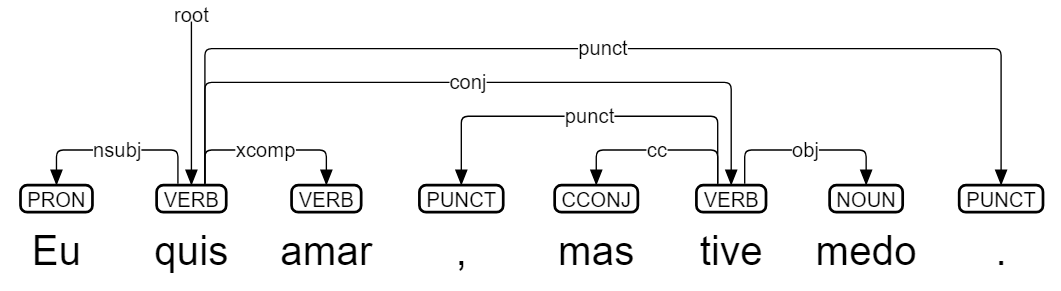
\includegraphics[scale=0.5]{images/lexicon_breakdown.png}
	\fautor
\end{figure}

A Análise de sentimentos emprega várias técnicas de \sigla{PLN}{Processamento de Linguagem Natural}, incluindo tokenização, lematização e remoção de palavras irrelevantes ou stop-words. A tokenização consiste em dividir o texto em palavras individuais ou "tokens". Já a lematização visa reduzir as palavras à sua forma base ou raiz, o que ajuda a consolidar diferentes formas da mesma palavra. Por sua vez, a remoção de palavras irrelevantes envolve a eliminação de termos comuns que geralmente não contribuem para o significado de uma frase, como "e", "o" e "em". Além dessas técnicas, a análise de sentimentos também se beneficia do uso de dicionários léxicos pré-existentes. Esses dicionários são valiosos recursos que contêm palavras associadas a valores de polaridade, indicando o sentimento geral de cada termo (positivo, negativo ou neutro).

\subsection{Dicionários léxicos}
\label{sec:dicionarios_lexicos}

No contexto da análise de sentimentos, existem vários dicionários léxicos relevantes disponíveis. Esse estudo comparou quatro repositórios bastante populares:

\begin{itemize}
	\item OpLexicon \cite{2011_Souza_IP}: É um dicionário léxico específico para o idioma português, com mais de 32.000 palavras, cada uma acompanhada de um valor de polaridade associado.
	\item SenticNet \cite{2016_Cambria_IP}: É dicionário léxico multilíngue que fornece valores de polaridade para palavras com base em sua semântica e psicologia.
	\item UniLex \cite{2017_Souza}: Outro dicionário léxico multilíngue que oferece valores de polaridade para palavras com base em uma variedade de recursos linguísticos.
	\item WordNetAffectBR \cite{2008_Pasqualotti}: Esta é uma versão em português do WordNet-Affect, um dicionário léxico que atribui valores de polaridade às palavras com base em sua associação com diferentes emoções.
\end{itemize}

Ao utilizar esses dicionários léxicos, podemos comparar as palavras presentes no texto com as entradas nos dicionários para determinar a polaridade de cada uma. Isso nos possibilita obter uma compreensão mais abrangente dos sentimentos expressos no texto, contribuindo para uma análise de sentimentos mais precisa e eficaz. Esses dicionários são ferramentas valiosas no campo da análise de sentimentos, auxiliando na identificação e interpretação das emoções presentes nas palavras utilizadas. Além disso, com base nesses recursos, é possível automatizar e ampliar a análise de sentimentos em textos extensos, como avaliações de produtos, publicações em redes sociais e outros tipos de conteúdo textual.

Durante a comparação da polaridade da frase de teste com os dicionários léxicos, notou-se uma discrepância na normalização dos dicionários Unilex e WordNetAffectBR. Para este experimento, optamos por utilizar apenas o OpLexicon e o SenticNet, devido aos seus scores similares de polaridade e à presença de palavras exclusivas em cada um desses dicionários.

Além disso, realizamos um teste utilizando um \textit{subset} dos dados das postagens do Colab para adequação ao contexto. Durante esse teste, identificamos palavras relevantes que não estavam presentes nos dicionários léxicos originais. Adicionamos manualmente essas palavras ao conjunto de dicionários, atribuindo-lhes scores de -1 a 1 com base na polaridade observada nas postagens do Colab.

Em seguida, realizamos uma análise comparativa para avaliar a eficácia desses dicionários léxicos. Durante essa análise, calculamos a polaridade resultante para cada um dos dicionários, buscando identificar qual deles é mais eficaz na análise de sentimentos no contexto específico das postagens do Colab. Como resultado, obtivemos um amalgama dos dicionários OpLexicon e SenticNet, além do conjunto de palavras que foram adicionadas manualmente. Essas palavras foram normalizadas e incorporadas ao processo de análise.

Durante a análise exploratória, observamos uma tendência intrigante: muitos usuários optavam por se comunicar usando emojis. Em algumas instâncias, os emojis eram usados para complementar o texto, enquanto em outras, eles eram a principal forma de expressão. Isso levantou a questão sobre a polaridade sentimental desses emojis. Para abordar essa questão, recorremos ao dataset de sentimentos de emojis criado por \citeonline{2015_Novak}. Este conjunto de dados oferece uma classificação de sentimentos para emojis comuns, permitindo-nos incorporar essa dimensão em nossa análise.

Além dos emojis, notamos a presença de jargões específicos frequentemente usados pelos usuários do aplicativo. Estes jargões, muitas vezes, carregavam um significado ou conotação que não era imediatamente claro para quem não estava familiarizado com o contexto do aplicativo. Reconhecendo a importância desses jargões na análise de sentimentos, decidimos classificar manualmente a polaridade dos 100 jargões mais comuns encontrados no app. Isso também incluiu a identificação e classificação de nomes de partidos políticos, dada a sua relevância no discurso dos usuários.

Outro aspecto que chamou nossa atenção foi a presença de profanidades nas postagens. A linguagem ofensiva ou abusiva pode ter um impacto significativo na polaridade de uma postagem. Portanto, introduzimos uma etapa adicional em nossa análise para detectar essas profanidades. Ao identificá-las, classificamos essas palavras com uma polaridade negativa, garantindo que sua presença influenciasse adequadamente o score de sentimento da postagem em questão. Com essas etapas adicionais, buscamos uma análise de sentimentos mais robusta e contextualizada, levando em consideração as peculiaridades e nuances do discurso dos usuários no aplicativo.

\subsection{Ferramenta LeIA}
\label{sec:ferramenta_leia}
Na busca por uma análise mais refinada e contextualizada dos sentimentos expressos nas postagens do Colab, decidimos incorporar uma métrica adicional ao nosso estudo: a análise de sentimentos realizada pelo pacote LeIA \cite{2018_Almeida_PAGE}. A inclusão dessa ferramenta visa aprimorar a nossa abordagem ao oferecer uma análise mais nuanceada dos sentimentos expressos nos textos, levando em consideração aspectos como a presença de emojis e a estrutura linguística das frases.

A ferramenta LeIA, desenvolvida especificamente para a língua portuguesa, apresenta uma abordagem que vai além da simples classificação de palavras individuais, oferecendo uma análise sintática e semântica mais profunda dos textos. Através da análise de sentimentos realizada pelo LeIA, obtemos uma pontuação composta (compound) que varia de -1 a +1, indicando o sentimento geral do texto, além de valores percentuais que representam a proporção de sentimentos positivos, negativos e neutros presentes no texto.

Para integrar essa métrica ao nosso estudo, adaptamos nossa função de análise de sentimentos para incluir a análise realizada pelo LeIA. Cada postagem do dataset foi analisada individualmente, gerando scores detalhados que incluem as métricas de positividade, negatividade, neutralidade e a pontuação composta. Esses scores foram então adicionados ao nosso dataset, prefixados com "leia" para indicar sua origem.

A decisão de integrar as métricas provenientes dos dicionários léxicos com as fornecidas pelo LeIA é motivada pela busca de uma análise mais holística e robusta. Enquanto nossos dicionários léxicos oferecem uma vasta base de palavras já classificadas, proporcionando uma análise ampla e generalizada, o LeIA traz uma perspectiva mais detalhada e contextual, capaz de interpretar nuances e particularidades da língua portuguesa, como a influência de emojis e a presença de negações no sentimento expresso. No entanto, é crucial reconhecer que tanto os dicionários léxicos quanto o LeIA podem introduzir seus próprios vieses na análise. Ao combinar essas métricas, aspiramos mitigar esses vieses individuais, buscando uma representação mais neutra e equilibrada dos sentimentos. A métrica composta, nesse contexto, não só permite uma categorização mais fluida dos sentimentos, evitando a rigidez das categorizações binárias, mas também proporciona uma visão mais matizada e imparcial dos dados.

Ao explorar a sinergia entre as métricas tradicionais e a análise realizada pelo LeIA, estamos em busca de respostas para uma questão central: como podemos, através da combinação de diferentes técnicas de análise de sentimentos, alcançar uma representação mais fiel e detalhada dos sentimentos expressos pelos usuários? Acreditamos que essa abordagem multidimensional pode revelar padrões e insights que seriam invisíveis através de uma única métrica. No entanto, é crucial enfatizar que a combinação de métricas apresenta desafios intrínsecos, sobretudo no que tange à calibração e à interpretação dos resultados. A integração das métricas não é uma simples concatenação de valores; ela demanda um processo meticuloso de normalização. Em nosso estudo, realizamos uma normalização dos scores para assegurar que as métricas provenientes de diferentes fontes estivessem em uma escala comum e comparável. Esse processo é fundamental para garantir que a combinação dos scores preserve a integridade e a precisão da análise, permitindo uma interpretação coesa e coerente dos sentimentos expressos nas postagens.

Para validar nossa abordagem, planejamos realizar uma série de testes e análises exploratórias, buscando entender como as métricas combinadas podem oferecer uma visão mais completa e rica dos sentimentos expressos nas postagens do Colab. Através dessa análise multidimensional, aspiramos a desvendar as complexidades do discurso dos usuários, oferecendo insights valiosos para a compreensão das dinâmicas sociais e emocionais presentes na plataforma.

Ao analisar a amostra fornecida, notamos que a combinação de métricas não apenas amplia a perspectiva sobre o sentimento, mas também ajuda a identificar nuances que poderiam ser perdidas se confiássemos em uma única métrica. Por exemplo, enquanto o score derivado dos dicionários léxicos pode capturar a polaridade geral de uma postagem, o leia\_compound do LeIA pode identificar sutilezas, como a influência de emojis ou a presença de negações, que podem alterar significativamente a interpretação do sentimento.

Além disso, observamos que a métrica composta compound\_score oferece uma visão mais equilibrada e matizada do sentimento. Em casos onde o score e o leia\_compound divergem, o compound\_score serve como uma espécie de "árbitro", proporcionando uma avaliação que leva em consideração ambas as perspectivas. Isso é particularmente útil em postagens onde o sentimento é ambíguo ou onde diferentes aspectos da postagem sugerem sentimentos contrastantes.

Outro insight interessante é a maneira como o compound\_score pode ajudar a identificar postagens que são particularmente polarizadas ou que geram sentimentos mistos. Postagens com compound\_scores próximos de zero, por exemplo, podem indicar postagens que contêm elementos tanto positivos quanto negativos, sugerindo que elas são mais complexas e merecem uma análise mais aprofundada.

Além disso, ao combinar métricas, também estamos abordando potenciais vieses inerentes a cada abordagem individual. Enquanto os dicionários léxicos podem ter suas próprias limitações e preconceitos, o LeIA, sendo uma ferramenta de aprendizado de máquina, pode ter seus próprios vieses com base nos dados com os quais foi treinado. Ao combinar essas métricas, esperamos criar uma métrica mais robusta e imparcial.

Em conclusão, ao adotar uma abordagem multidimensional para a análise de sentimentos, estamos não apenas buscando uma representação mais precisa do sentimento, mas também tentando entender as complexidades e nuances do discurso dos usuários. Esta abordagem combinada promete oferecer insights mais ricos e detalhados, permitindo uma compreensão mais profunda das emoções e opiniões expressas na plataforma Colab.

\section{Máquina e Regressão Supervisionada}

A aprendizagem de máquina, uma vertente fundamental da inteligência artificial, tem revolucionado diversos campos de pesquisa e aplicação prática. Esta área foca no desenvolvimento de algoritmos capazes de aprender e aprimorar-se automaticamente a partir de dados, sem programação direta e explícita. \citeonline{2017_Goodfellow_BOOK} destacam a importância do aprendizado de máquina na pesquisa de inteligência artificial, salientando sua capacidade de adaptar-se e evoluir com novas informações.

No âmbito do aprendizado supervisionado, um dos pilares do aprendizado de máquina, os algoritmos são treinados usando conjuntos de dados rotulados. Este método é essencial para ensinar máquinas a fazer previsões ou classificações precisas com base em dados de entrada. Segundo \citeonline{2017_Shen}, a distinção entre classificação e regressão é crucial no aprendizado supervisionado, com a regressão focando em prever saídas contínuas e a classificação em categorizar dados em classes discretas.

A regressão supervisionada, em particular, é usada para prever resultados contínuos, sendo uma ferramenta poderosa em campos como a análise de sentimento, onde as emoções humanas são mapeadas em um espectro contínuo. Esta abordagem reconhece a natureza graduada e multidimensional dos sentimentos, contrastando com métodos mais simplistas que categorizam emoções em binários positivos ou negativos \cite{2023_Patrick_IP}.

Dentro deste contexto, a análise de sentimento emerge como uma aplicação significativa do aprendizado de máquina. Através dela, sentimentos expressos em textos podem ser quantificados e analisados, oferecendo insights valiosos para diversas áreas, desde o marketing até a política. Esta técnica ilustra a capacidade do aprendizado de máquina de interpretar e processar linguagem natural, um desafio complexo que está no coração da interação entre humanos e máquinas. Por exemplo, \citeonline{2021_Matalon} analisaram um corpus de 715.894 tweets em inglês relacionados ao conflito israelense-palestino. Neste estudo, foi desenvolvido um modelo de classificação de polaridade em relação a Israel, classificando cada tweet em categorias de suporte, neutralidade ou oposição. Este trabalho destacou a capacidade do aprendizado de máquina em interpretar e processar a linguagem natural, demonstrando a eficácia da análise de sentimentos em um contexto político complexo e emocionalmente carregado.

Essas tecnologias, impulsionadas pelas inovações em redes neurais e aprendizado profundo, continuam a expandir as fronteiras do que as máquinas podem aprender e realizar. \citeonline{1999_Haykin_BOOK} enfatiza a importância das redes neurais na prática e teoria do aprendizado de máquina, destacando como elas são fundamentais para o avanço da inteligência artificial. Nesse sentido, o aprendizado de máquina e a regressão supervisionada representam não apenas ferramentas tecnológicas avançadas, mas também janelas para compreender os aspectos humanos de percepção e cognição, criando um campo de estudo que é tão rico em possibilidades quanto desafiador em suas complexidades.

Em conclusão, é importante salientar que empregaremos a técnica de regressão supervisionada como uma metodologia central no nosso estudo para classificar postagens. Essa abordagem é particularmente eficaz para a análise de sentimentos, pois permite capturar nuances e graduações nos sentimentos expressos em textos. Ao invés de simplificar a complexidade dos sentimentos humanos em categorias binárias, a regressão supervisionada oferece um espectro contínuo que reflete mais precisamente as variações e a riqueza das expressões emocionais.

Neste contexto, a classificação de postagens através da regressão supervisionada não só contribui para uma melhor compreensão dos sentimentos e opiniões expressos em plataformas digitais, mas também amplia nosso entendimento sobre como as pessoas se comunicam e interagem em ambientes online. Ao aplicar este método em nossa análise de sentimentos, esperamos extrair insights valiosos que vão além do que é possível com abordagens de classificação tradicionais, fornecendo uma perspectiva mais rica e detalhada sobre a dinâmica das comunicações humanas na era digital.

Portanto, o uso da regressão supervisionada no estudo não é apenas uma escolha metodológica, mas também um passo em direção a uma análise mais aprofundada e humanizada das interações online, refletindo a complexidade e a profundidade dos sentimentos humanos. Os experimentos de análise de sentimentos são detalhados em \autoref{sec:analise_de_sentimento_com_regressao_supervisionada}.

\subsection{Avaliação do desempenho de modelos de regressão}

Para assegurar a eficácia e a precisão dos modelos de análise de sentimentos em postagens, é essencial empregar métricas de avaliação de desempenho específicas. Estas métricas, fundamentais para entender a reação do modelo a diferentes tipos de dados e garantir previsões confiáveis, são detalhadamente exploradas no trabalho de \citeonline{2023_SHUKLA_PAGE}. As técnicas empregadas, como \sigla{$MSE$}{Mean Squared Error}, \sigla{$MAE$}{Mean Absolute Error} e \sigla{$R2$}{Coeficiente de Determinação}, são cruciais para avaliar a precisão e eficácia das previsões do modelo. As definições e discussões sobre estas métricas e outros conceitos relevantes ao aprendizado de máquina supervisionado apresentadas nos parágrafos a seguir são baseadas nas análises abrangentes de Shukla, cujo trabalho ganhou destaque e popularidade online, refletido nos milhares de compartilhamentos e em uma tradução em português realizada por Acervo Lima\footnote{\url{https://acervolima.com/regressao-e-classificacao-aprendizado-de-maquina-supervisionado/}}.

O $MSE$ é uma medida do erro quadrático médio entre as previsões do modelo e os sentimentos reais das postagens. Em análise de sentimentos, um $MSE$ baixo indica que o modelo é capaz de prever sentimentos de maneira precisa, com um pequeno desvio em relação aos valores reais. No entanto, devido à sua tendência de dar maior peso a outliers, é necessário ter cautela ao interpretar o $MSE$, principalmente em conjuntos de dados com variações extremas de sentimentos.

Por sua vez, o $MSE$ fornece uma medida mais intuitiva do erro médio absoluto entre as previsões e os sentimentos reais. Sendo menos sensível a outliers do que o $MSE$, o $MAE$ é particularmente útil na análise de sentimentos quando se deseja evitar que postagens atípicas distorçam a avaliação do modelo. Um $MAE$ baixo sugere que o modelo, em média, faz previsões que estão próximas do sentimento real, independentemente de variações extremas nas postagens.

Além disso, o Coeficiente de Determinação, R\^2, é usado para medir quão bem as previsões do modelo correspondem aos sentimentos reais das postagens. Um valor alto de R\^2 indica que uma grande proporção da variação nos sentimentos é explicada pelo modelo, o que é desejável em análise de sentimentos. Isso significa que o modelo é eficaz em captar a essência dos sentimentos expressos nas postagens, refletindo uma boa adaptação do modelo aos dados.

Essas métricas, quando combinadas, oferecem uma visão abrangente da performance do modelo de análise de sentimentos. Elas permitem avaliar não só a precisão global do modelo, mas também sua capacidade de lidar com variações e dados atípicos. A escolha  e interpretação corretas destas métricas são cruciais para garantir a confiabilidade e aplicabilidade do modelo na análise de sentimentos em postagens.

\section{Classificação Supervisionada}

No campo do aprendizado de máquina, a classificação supervisionada desempenha um papel crucial ao permitir que os algoritmos categorizem dados em classes pré-definidas, utilizando dados rotulados para treinar modelos. Estes modelos são, então, capazes de classificar novas instâncias com base no aprendizado adquirido. A classificação supervisionada se distingue da regressão supervisionada, que foca na previsão de variáveis contínuas, ao passo que a classificação lida com categorias discretas. Segundo uma análise apresentada por \citeonline{2023_SHUKLA_PAGE}, a principal diferença entre essas duas tarefas é que, enquanto a regressão lida com um atributo dependente numérico, a classificação trabalha com um atributo dependente categórico.

A classificação é utilizada para atribuir categorias a pontos de dados com valores discretos. Por exemplo, um modelo de classificação pode ser usado para determinar se um nome é masculino ou feminino, ou categorizar e-mails como 'spam' ou 'não spam'. Essa distinção é crucial, pois a classificação produz valores discretos e define dados em categorias estritas, ao contrário da regressão, que busca distinguir entre pontos individuais em um espectro contínuo.

No campo do aprendizado de máquina, a classificação supervisionada é uma técnica central que permite aos algoritmos aprenderem a categorizar dados em classes pré-definidas. Entre os algoritmos mais conhecidos para essa tarefa, podemos destacar o \sigla{$KNN$}{K-Nearest Neighbors}, a Regressão Logística e as \sigla{SVM}{Máquinas de Vetores de Suporte}.

O $KNN$ é um algoritmo baseado na ideia de que instâncias semelhantes tendem a estar próximas umas das outras. Em outras palavras, ele classifica um ponto de dados com base em como seus vizinhos estão categorizados. Esse método é eficaz, mas pode se tornar menos eficiente à medida que o volume de dados aumenta \cite{2011_Samworth}.

A Regressão Logística, por sua vez, é amplamente utilizada em classificação binária. Apesar de seu nome, não é usada para prever eventos logísticos, mas sim para classificação com base na função logística. Este modelo é valorizado por sua simplicidade e capacidade de lidar eficientemente com grandes conjuntos de dados \cite{2010_Yu}.

Por fim, as $SVM$ são conhecidas por sua eficácia em espaços de alta dimensão e por sua capacidade de criar hiperplanos que maximizam a margem entre as classes de dados. Esse algoritmo é particularmente útil em situações onde a distinção entre as classes não é muito clara \cite{2004_Smola}.

Cada um desses algoritmos tem características únicas e se adequa a diferentes tipos de problemas de classificação. A escolha do algoritmo mais apropriado depende da natureza específica do problema e dos dados disponíveis. A compreensão desses algoritmos e sua aplicação correta são fundamentais para resolver problemas complexos de classificação no campo do aprendizado de máquina.

Um aspecto crucial no desenvolvimento de modelos de classificação é a consideração de problemas como overfitting e underfitting. O overfitting, conforme descrito no trabalho de \citeonline{2020_Bashir}, ocorre quando um modelo se ajusta excessivamente aos detalhes e ruídos dos dados de treinamento, prejudicando sua capacidade de generalização para novos dados. Por outro lado, underfitting acontece quando um modelo é demasiadamente simples e não aprende o suficiente sobre a estrutura dos dados de treinamento, falhando em capturar padrões importantes. Estes desafios podem ser superados com o uso apropriado de técnicas de validação e regularização, como LASSO e Ridge, que ajudam a equilibrar a complexidade do modelo e sua precisão na previsão de novos dados.

\citeonline{2019_Ying} discute várias estratégias para mitigar o overfitting em modelos de aprendizado de máquina supervisionado, propondo soluções como "early-stopping", que interrompe o treinamento antes da otimização completa; "network-reduction", para excluir ruídos do conjunto de treinamento; "data-expansion", para ajustar hiperparâmetros em modelos complexos com uma grande quantidade de dados; e "regularização", que ajuda a selecionar características e diferenciar as mais e menos úteis.

Estas soluções são aplicadas no contexto do nosso estudo para assegurar que os modelos de classificação de postagens, especialmente em análise de sentimentos, sejam precisos e eficazes, evitando tanto o overfitting quanto o underfitting. A aplicação dessas técnicas é crucial para o balanceamento da complexidade do modelo e sua precisão na previsão

\subsection{Avaliação do desempenho de modelos de classificação}

Ao desenvolver modelos para análise de sentimentos, é essencial empregar métodos robustos de avaliação de desempenho. Entre esses, a curva ROC (Receiver Operating Characteristic) e a análise da área sob a curva (AUC), junto com a validação cruzada, são técnicas cruciais.

A curva ROC é uma ferramenta gráfica usada para avaliar a capacidade de um modelo de classificação em distinguir entre classes. Em análise de sentimentos, isso se traduz em quão bem o modelo pode diferenciar entre sentimentos positivos, negativos e neutros. A curva é plotada com a taxa de verdadeiros positivos (sensibilidade) no eixo Y contra a taxa de falsos positivos (especificidade) no eixo X. Um modelo perfeito seguiria o canto superior esquerdo do gráfico, indicando uma alta sensibilidade sem falsos positivos. A curva ROC é particularmente útil em ambientes com um desequilíbrio significativo de classes, que é comum em análises de sentimentos de dados de redes sociais ou de avaliações de clientes.

A análise AUC, por sua vez, proporciona uma medida quantitativa da capacidade do modelo de classificação. AUC representa a área sob a curva ROC. Um valor de AUC de 1.0 indica um modelo perfeito, enquanto um valor de 0.5 sugere um desempenho não melhor que um chute aleatório. Em análise de sentimentos, um alto valor de AUC indica que o modelo tem uma boa capacidade de distinguir entre diferentes sentimentos, o que é crucial para aplicações práticas como monitoramento de marca ou análise de feedback de clientes.

Além destas métricas, a validação cruzada é uma técnica de avaliação do modelo que visa garantir que o modelo seja generalizável e não apenas ajustado ao conjunto de dados de treinamento. A validação cruzada estratificada, ou stratified k-fold, é uma variação que garante que cada dobra (fold) de dados tenha a mesma proporção de classes que o conjunto de dados original. Isso é especialmente importante em análises de sentimentos, onde a distribuição de sentimentos pode variar significativamente. Por exemplo, em um conjunto de dados com uma grande maioria de sentimentos positivos, a validação cruzada estratificada garante que cada dobra tenha uma representação proporcional de sentimentos positivos, negativos e neutros.

A combinação dessas técnicas proporciona uma avaliação abrangente e confiável do modelo de análise de sentimentos. Enquanto a curva ROC e a análise AUC oferecem insights sobre a capacidade discriminatória do modelo, a validação cruzada estratificada assegura que a avaliação seja equitativa e representativa do conjunto de dados em geral. Por exemplo, \citeonline{2022_Ogbuokiri} mostrou o desempenho de diferentes classificadores de sentimentos de tweets, como regressão logística e SVM, usando a curva ROC e a análise AUC para avaliar sua eficácia. Este estudo ressalta a importância da aplicação de técnicas de avaliação como ROC-AUC em contextos de análise de sentimentos, onde a precisão na classificação dos sentimentos é crucial para uma interpretação correta e insights valiosos.

Essas técnicas, quando aplicadas corretamente, proporcionam uma compreensão profunda da eficácia do modelo de análise de sentimentos. A curva ROC e a análise AUC permitem uma avaliação visual e numérica da capacidade do modelo de distinguir entre diferentes categorias de sentimentos. Ao mesmo tempo, a validação cruzada estratificada assegura que o modelo seja robusto e confiável, não apenas para o conjunto de dados em que foi treinado, mas também para novos dados que possam ser encontrados em aplicações práticas.

Para implementar essas técnicas de forma eficaz, é essencial compreender a natureza dos dados de análise de sentimentos e as peculiaridades do modelo de aprendizado de máquina utilizado. A escolha de parâmetros, o equilíbrio entre a complexidade do modelo e a prevenção de overfitting ou underfitting, e a interpretação correta das métricas de desempenho são etapas cruciais que determinam o sucesso da análise de sentimentos.

Em resumo, a integração da curva ROC, análise AUC e validação cruzada estratificada em análise de sentimentos proporciona uma avaliação abrangente e confiável, fundamental para desenvolver modelos precisos e eficazes em uma variedade de aplicações práticas. Essas técnicas não apenas garantem a qualidade do modelo, mas também fornecem insights valiosos para aprimoramentos contínuos e ajustes no modelo para lidar com diferentes tipos de dados de sentimentos.



\section{Modelagem Baseada em Agentes}
\label{05_mba}
A Modelagem Baseada em Agentes (MBA) é uma abordagem de modelagem computacional que permite simular e analisar sistemas complexos através da interação de agentes autônomos. Essa abordagem tem sido aplicada em diversos campos, como ciências sociais, economia, ecologia e engenharia, devido à sua capacidade de capturar comportamentos emergentes e padrões coletivos resultantes das interações entre os agentes.

No contexto específico das simulações de câmaras de eco, a MBA oferece uma poderosa ferramenta para investigar e compreender a dinâmica desses sistemas. As câmaras de eco são ambientes onde grupos de indivíduos compartilham e são expostos principalmente a informações e opiniões que confirmam suas crenças existentes, resultando em polarização e reforço de pontos de vista extremos. Utilizando a MBA, é possível modelar os usuários como agentes autônomos, considerando suas opiniões individuais, influências externas e interações em uma rede social.

Ao simular a interação e a propagação de informações entre os agentes, é possível estudar como as câmaras de eco se formam e evoluem, analisando os fatores que contribuem para a polarização e a formação de bolhas de informação. A MBA permite investigar diferentes estratégias de atualização de opinião dos agentes, a influência dos vizinhos na rede social e outros fatores que afetam a dinâmica das câmaras de eco. Além disso, é possível utilizar medidas e métricas para avaliar o impacto das câmaras de eco, como a diversidade de opiniões, a polarização e a exposição a diferentes perspectivas.

Portanto, a Modelagem Baseada em Agentes é uma valiosa ferramenta para compreender e analisar as dinâmicas das câmaras de eco. Ao simular a interação dos agentes em um ambiente controlado, é possível obter insights sobre os processos subjacentes e os efeitos resultantes das câmaras de eco. Essa abordagem permite explorar estratégias de mitigação e intervenção para promover a diversidade de opiniões e evitar o reforço de extremos, contribuindo para uma sociedade mais plural e informada.

Exploramos a metodologia proposta por Atiqi, focando na simulação da dinâmica de opiniões em uma rede social. O modelo de simulação é baseado em agentes, em que cada agente representa um usuário na rede social. Cada usuário possui uma opinião e uma exposição, que são atualizadas com base nas notícias que encontram e nas opiniões de seus vizinhos na rede.

A opinião de um usuário é um valor entre -1 e 1, representando o sentimento do usuário em relação a um determinado tópico. A exposição de um usuário é uma medida da diversidade de sentimentos das notícias que encontraram. Ela aumenta sempre que um usuário encontra uma notícia cujo sentimento é diferente de sua opinião atual.

O modelo de simulação utiliza diferentes estratégias para atualizar as opiniões dos usuários. A estratégia básica atualiza a opinião de um usuário com base no sentimento de uma notícia, se a diferença entre a opinião do usuário e o sentimento da notícia estiver abaixo de um determinado limite. Estratégias mais complexas também levam em consideração as opiniões dos vizinhos do usuário na rede. Por exemplo, a estratégia de Influência do Vizinho atualiza a opinião de um usuário em direção à opinião média de seus vizinhos se suas opiniões tiverem o mesmo sinal. A estratégia de Influência do Vizinho Ponderada faz o mesmo, mas pondera as opiniões dos vizinhos pela centralidade do eigenvector na rede.

Estratégia \texttt{NeighborInfluenceOpinionUpdateStrategy}:
\begin{equation*}
	O_i = O_i + \alpha \times (M_i - O_i)
\end{equation*}

em que:

\begin{itemize}
	\item $O_i$ representa a opinião do usuário $i$;
	\item $M_i$ representa a média das opiniões dos vizinhos do usuário $i$;
	\item $\alpha$ é o fator de influência que determina o quanto a opinião dos vizinhos influencia a opinião do usuário.
\end{itemize}

Estratégia \texttt{WeightedNeighborInfluenceOpinionUpdateStrategy}:
\begin{equation*}
	O_i = O_i + \alpha \times (M_{\text{ponderada}_i} - O_i)
\end{equation*}

em que:

\begin{itemize}
	\item $O_i$ representa a opinião do usuário $i$;
	\item $M_{\text{ponderada}_i}$ representa a média ponderada das opiniões dos vizinhos do usuário $i$;
	\item $\alpha$ é o fator de influência que determina o quanto a opinião ponderada dos vizinhos influencia a opinião do usuário.
\end{itemize}

A simulação produz várias métricas que podem ser usadas para analisar a dinâmica da rede:

\begin{itemize}
	\item Coeficiente Global de Câmaras de Eco (GEC): uma medida que quantifica a polarização de opiniões na rede. O GEC é calculado somando o produto das opiniões dos pares de usuários conectados por uma aresta na rede. Um valor positivo indica uma tendência de polarização, em que usuários com opiniões semelhantes estão mais propensos a se conectar entre si, enquanto um valor negativo indica uma tendência de diversidade de opiniões.
	\item Coeficiente Individual de Câmaras de Eco (ECC): uma medida que avalia a polarização de opiniões com base na diversidade de exposição a diferentes perspectivas. O ECC é calculado para cada usuário, considerando as opiniões dos seus vizinhos na rede. Um valor alto de ECC indica que um usuário está principalmente exposto a opiniões semelhantes à sua, refletindo a existência de câmaras de eco.
	\item Opinião Média: uma medida que representa a opinião média dos usuários na rede. É calculada como a média das opiniões individuais de todos os usuários. A opinião média fornece uma visão geral do sentimento coletivo em relação a um determinado tópico na rede.
	\item Exposição Média: uma medida que representa a exposição média dos usuários a diferentes perspectivas na rede. É calculada como a média das exposições individuais de todos os usuários. A exposição média reflete a diversidade de informações a que os usuários estão expostos e pode indicar o grau de pluralismo de opiniões na rede.
\end{itemize}

Considerando as heurísticas propostas em um contexto de simulação e as condições únicas dos dados do Colab, representando tanto uma topologia de grafo de rede social quanto o conteúdo produzido por usuários dessa rede, metodologia de Atiqi fornece um framework poderoso para simular e analisar a dinâmica de opiniões no Colab. O modelo baseado em agentes permite uma representação detalhada dos usuários e suas interações, enquanto as diversas métricas e visualizações proporcionam insights sobre a dinâmica da rede. No entanto, interpretar esses resultados de maneira significativa muitas vezes requer compará-los a outros resultados, seja de outras simulações ou de dados do mundo real. Nossa intenção é adaptar a metodologia de Atiqi para o caso de uso do Colab, substituindo as notícias por eventos reportados pelos usuários e as opiniões por sentimentos expressos nos comentários/postagens. Dessa forma, poderemos simular a dinâmica de opiniões e a formação de câmaras de eco no contexto do aplicativo Colab. Exploramos essas dinâmicas no \autoref{chapter:08_echochamberdetection}.

\section{Conclusões}
Neste capítulo de Fundamentação Teórica, exploramos conceitos e teorias essenciais que fornecem uma base sólida para a compreensão das dinâmicas das câmaras de eco em redes sociais, com foco na aplicação desses conceitos ao contexto do aplicativo Colab. Começamos introduzindo a teoria dos grafos e sua relevância na representação de redes sociais, destacando a importância da detecção de comunidades e da modularidade para identificar estruturas significativas dentro dessas redes. Em seguida, discutimos o algoritmo Louvain, uma técnica eficaz para a detecção de comunidades em redes complexas, que desempenhará um papel fundamental em nossas análises.

Em seguida, investigamos as aplicações da análise de redes sociais em diversos campos, reconhecendo a importância dessa abordagem na compreensão das dinâmicas das redes e na identificação de padrões emergentes. Exploramos as câmaras de eco e suas implicações nas mídias sociais, destacando como esses fenômenos podem levar à polarização e à disseminação de desinformação.

Examinamos as implicações negativas das câmaras de eco, incluindo a dificuldade de diálogo construtivo, a disseminação de desinformação e a fragmentação da sociedade. Investigamos os mecanismos por trás da formação das câmaras de eco, que envolvem algoritmos de personalização de conteúdo, vieses cognitivos e influência de líderes de opinião.

Destacamos a importância de compreender esses mecanismos para mitigar os efeitos negativos das câmaras de eco, especialmente no contexto do aplicativo Colab. Analisamos estudos relevantes que examinaram câmaras de eco em diferentes contextos, incluindo política climática e debates sobre vacinação.

Finalmente, introduzimos a Modelagem Baseada em Agentes (MBA) como uma ferramenta poderosa para simular a dinâmica das câmaras de eco. A MBA permite a criação de simulações que representam a interação de agentes autônomos, que são os usuários de redes sociais. Exploramos um modelo de simulação baseado em MBA que pode ser adaptado ao contexto do Colab, permitindo-nos investigar como as câmaras de eco podem se formar e evoluir dentro da plataforma.

Nos próximos capítulos, daremos um passo adiante na nossa jornada de compreensão das câmaras de eco no aplicativo Colab. Esperamos que a base teórica oferecida nesse capítulo ilumine e informe a metodologia aplicada nos próximos passos. De maneira geral a intenção foi demonstrar como soluções matemáticas para problemas analógicos como as Pontes de Königsberg fornecem um framework para análises digitais e de dinâmicas sociais Usando a poderosa ferramenta Gephi, realizaremos uma análise exploratória da rede do Colab. Iremos visualizar e examinar a estrutura da rede, identificar comunidades e padrões de interação, e começar a descobrir insights sobre como as câmaras de eco podem estar se formando na plataforma. Esta análise nos proporcionará uma base sólida para investigações mais aprofundadas e a formulação de estratégias para lidar com os desafios das câmaras de eco no Colab.